% !TEX program = xelatex
\documentclass[11pt,a4paper]{article}
\usepackage[numbers,sort&compress]{natbib}
\usepackage{geometry}
\usepackage{fontspec} 
\usepackage{underscore}
\usepackage{hyperref}
\usepackage{mathtools}
\usepackage{pdfpages}

\setmainfont{Cambria}
\geometry{letterpaper,scale=0.95}
%%%%%%%%%
\begin{document}
\newpage
\begin{minipage}[t][500pt]{0.2\linewidth}
\paragraph{Cues:}
\begin{itemize}
    \item Point A
    \item Point B
    \item Point C
    \item Point D
\end{itemize}    
\end{minipage}
\hfill
\begin{minipage}[t][500pt]{0.65\linewidth}
    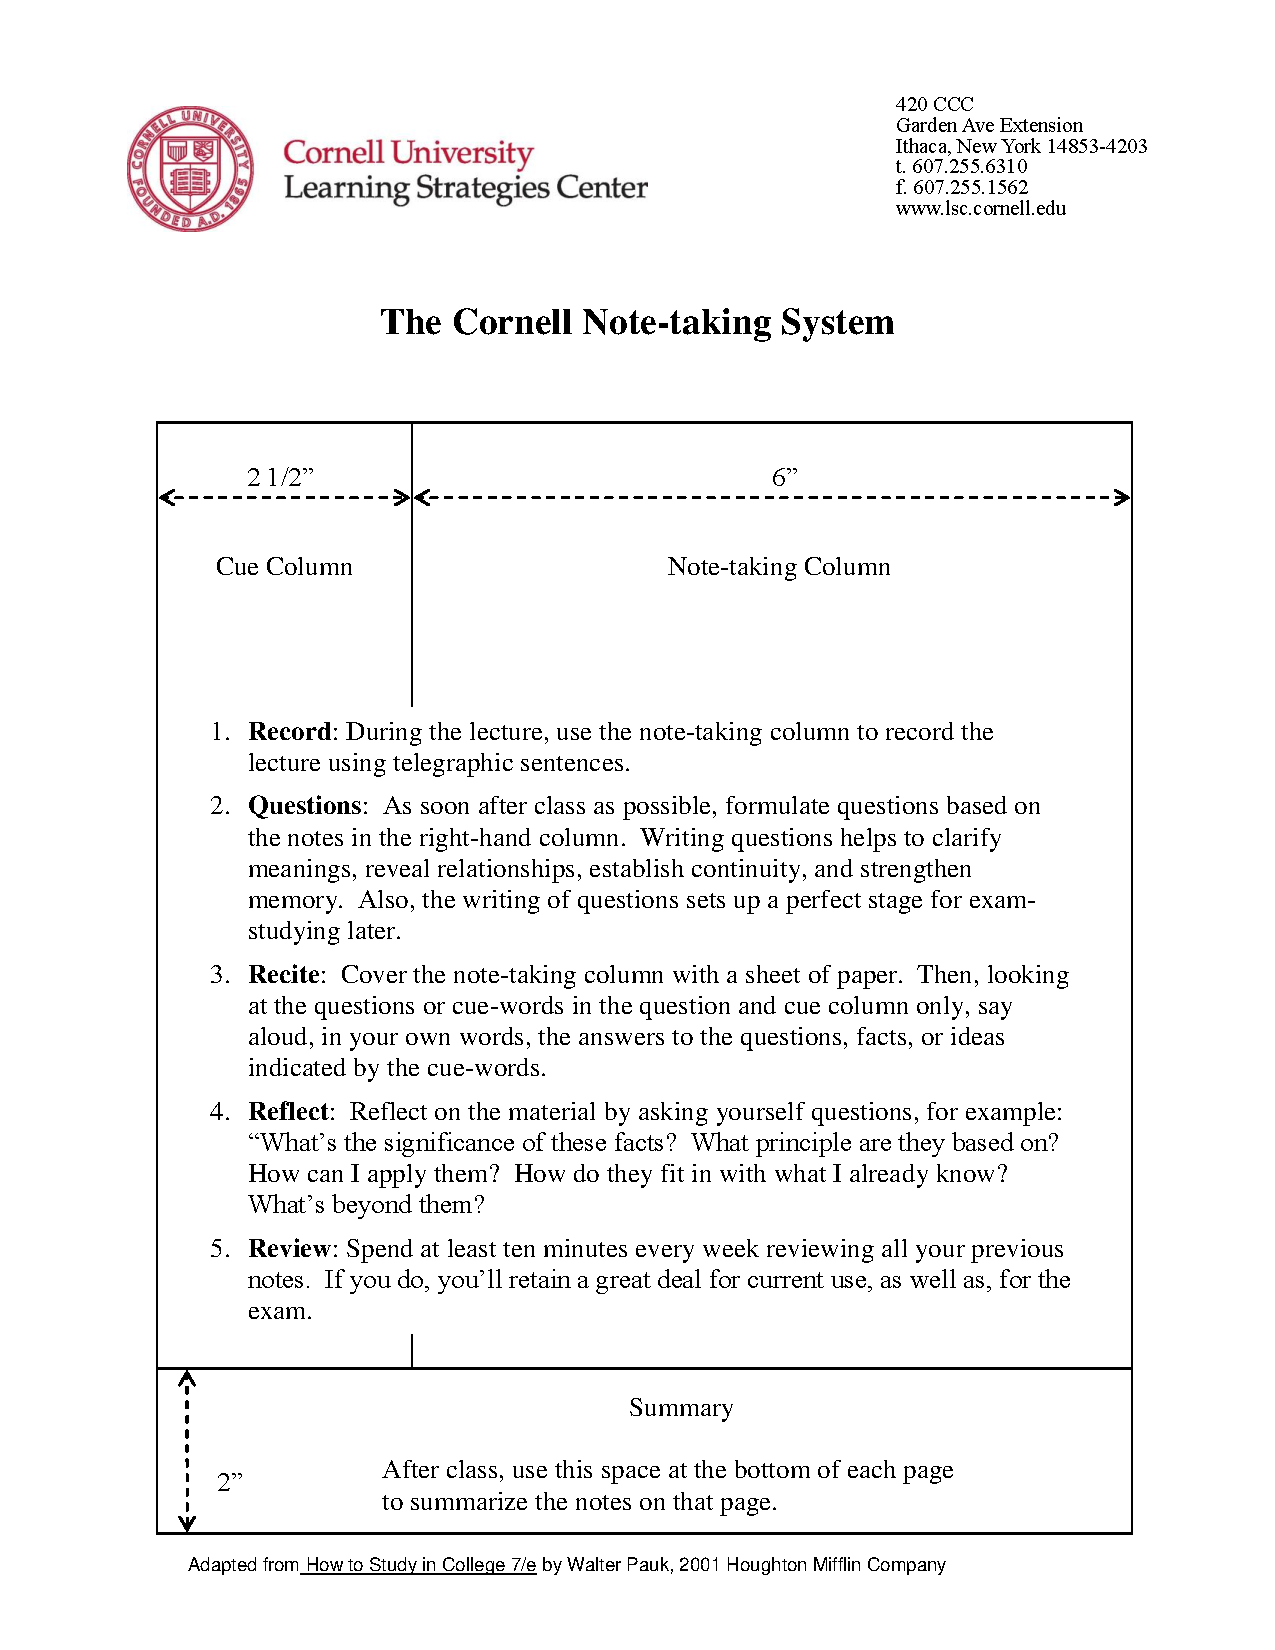
\includepdf[pages={1},width=0.8\linewidth]{example.pdf} %pages = {<the page you want to add cues>}
\end{minipage}
\vfill
\rule{0.95\linewidth}{0.05em}

\begin{minipage}[t][150pt]{\linewidth}
\paragraph{Conclusion:}
????
\end{minipage}

\end{document}